\documentclass[11pt]{article}
\usepackage[a4paper,margin=2.3cm]{geometry}
\usepackage{amsmath,amssymb}
\usepackage{graphicx}
\usepackage{booktabs}
\usepackage{xcolor}
\usepackage{titlesec}
\usepackage{caption}
\usepackage{hyperref}
\usepackage{array}
\usepackage{enumitem}
\usepackage{fancyhdr}

\definecolor{edhecred}{RGB}{158,27,50}
\definecolor{edhecgray}{RGB}{77,77,77}

\titleformat{\section}{\large\bfseries\color{edhecred}}{\thesection}{0.6em}{}
\titleformat{\subsection}{\normalsize\bfseries\color{edhecgray}}{\thesubsection}{0.6em}{}
\hypersetup{colorlinks=true, linkcolor=edhecred, urlcolor=edhecred, citecolor=edhecred}

\graphicspath{{outputs/}{ga_project/outputs/}{python_labs/outputs/}}

\pagestyle{fancy}
\fancyhf{}
\lhead{\small Advanced Fixed Income and Credit --- Group Assignment}
\rhead{\small\thepage}
\renewcommand{\headrulewidth}{0.3pt}

\newcommand{\question}[1]{\subsection*{\textcolor{edhecred}{#1}}}

\begin{document}

%====================================================================
\begin{titlepage}
\centering
\vspace*{2cm}
{\LARGE\bfseries\color{edhecred} Advanced Fixed Income and Credit}\\[0.4cm]
{\Large Group Assignment}\\[1.2cm]
{\large Part I: Deutsche Bank --- Finding Relative-Value Trades (HBS 205-059)}\\
{\large Part II: Python Labs --- US Treasury Yield Curve Reaction to Trump Tariff Threats}\\[2cm]
{\large EDHEC Business School --- MSc\\ Advanced Fixed Income and Credit, Thibault Lair}\\[2cm]
{\large \today}\\[1cm]
\vfill
{\small \textit{Group members: [FILL IN NAMES HERE]}}
\end{titlepage}

\tableofcontents
\newpage

%====================================================================
\section{Part I --- The Deutsche Bank Case Study}

\subsection*{Setup and conventions}
Settlement date: \textbf{August 15, 2003}. Exhibit 1 lists 52 Treasury coupon
bonds whose maturities fall on successive semi-annual dates (Feb 15 / Aug 15)
from 2004 to 2029 with no gaps, i.e.\ exactly one bond at each of the nodes
$t=0.5,1.0,\dots,26.0$ years. This allows the classic \emph{successive
substitution} bootstrap: because each bond introduces exactly one new unknown
discount factor, we solve sequentially from the shortest to the longest
maturity.

\textbf{Compounding convention.} Exhibit 4's footnote states explicitly that
Deutsche Bank's own model yields are \emph{Bond-Equivalent Yields} (BEY),
i.e.\ twice the semi-annual compounded yield. Since U.S.\ Treasuries pay
semi-annual coupons, we derive our own zero-coupon yields in the identical
BEY convention throughout, so that every comparison against the DB model in
Q1.2 is apples-to-apples (a continuously-compounded convention would have
introduced a small but systematic bias in one direction).
$$\text{BEY} = 2\left(D^{-1/k}-1\right), \qquad D = \text{discount factor to period } k \text{ (6-month steps)}.$$

%--------------------------------------------------------------------
\question{Q1.1 --- Bootstrapping the discount curve}

\textbf{Methodology.} For bond $k$ (maturing at period $k$, coupon $c$ per
annum, price $P_k$):
$$P_k = \frac{c}{2}\sum_{j=1}^{k-1} D_j + \left(\frac{c}{2}+100\right)D_k
\quad\Longrightarrow\quad
D_k = \frac{P_k - \frac{c}{2}\sum_{j=1}^{k-1}D_j}{\frac{c}{2}+100}.$$
Solved in order of increasing maturity, using only already-known $D_j$, $j<k$.

\textbf{Validation.} Our bootstrapped curve matches Deutsche Bank's own
Exhibit 4 model yields \emph{exactly} at 2Y (1.873\%) and 10Y (4.711\%) ---
precisely the maturities the case identifies as DB's own calibration points
for its three-factor model. This is strong internal validation that both the
bootstrap algorithm and the BEY convention choice are correct.

\begin{table}[h]
\centering
\small
\begin{tabular}{rrrr}
\toprule
Maturity (y) & Discount Factor & Zero Yield (BEY) \\
\midrule
0.5  & 0.99561 & 0.882\% \\
1.0  & 0.98818 & 1.193\% \\
2.0  & 0.96341 & 1.873\% \\
5.0  & 0.84156 & 3.480\% \\
10.0 & 0.62775 & 4.711\% \\
15.0 & 0.42935 & 5.717\% \\
20.0 & 0.30947 & 5.951\% \\
25.0 & 0.23299 & 5.913\% \\
26.0 & 0.22024 & 5.905\% \\
\bottomrule
\end{tabular}
\caption{Bootstrapped zero-coupon curve, selected maturities (full 52-point curve in \texttt{q1\_bootstrapped\_curve.csv}).}
\end{table}

The curve shape is the standard concave, upward-sloping Treasury curve of
the period, flattening from about 15Y onward and showing a very slight
downward drift between 20Y and 26Y.

%--------------------------------------------------------------------
\question{Q1.2 --- Comparison with Deutsche Bank's model, trading signals}

\textbf{Logic.} Yield and price move in opposite directions. If our
bootstrapped (market-implied) yield is \emph{higher} than DB's model yield,
the bond's market price is below the model's ``fair'' price $\Rightarrow$ the
bond is \textbf{cheap} $\Rightarrow$ \textbf{BUY}. If the market yield is
\emph{lower}, the bond is \textbf{rich} $\Rightarrow$ \textbf{SELL}.

\begin{table}[h]
\centering
\small
\begin{tabular}{rrrrl}
\toprule
Maturity (y) & DB Model Yield & Market Yield (Q1.1) & Diff (bps) & Signal \\
\midrule
1  & 1.2443\% & 1.1930\% & $-5.13$ & SELL (rich) \\
2  & 1.8727\% & 1.8727\% & $+0.00$ & fair (DB calibration point) \\
3  & 2.4110\% & 2.4711\% & $+6.01$ & \textbf{BUY (cheap)} \\
4  & 2.9665\% & 3.0084\% & $+4.19$ & \textbf{BUY (cheap)} \\
5  & 3.4454\% & 3.4799\% & $+3.45$ & \textbf{BUY (cheap)} \\
6  & 3.8557\% & 3.8817\% & $+2.60$ & \textbf{BUY (cheap)} \\
7  & 4.1996\% & 4.2203\% & $+2.07$ & \textbf{BUY (cheap)} \\
8  & 4.4677\% & 4.4865\% & $+1.88$ & \textbf{BUY (cheap)} \\
9  & 4.6528\% & 4.6640\% & $+1.12$ & \textbf{BUY (cheap)} \\
10 & 4.7107\% & 4.7107\% & $-0.00$ & fair (DB calibration point) \\
15 & 5.7160\% & 5.7167\% & $+0.07$ & fair \\
20 & 5.9517\% & 5.9513\% & $-0.04$ & fair \\
25 & 5.9315\% & 5.9128\% & $-1.87$ & SELL (rich) \\
\bottomrule
\end{tabular}
\caption{Market vs. DB model comparison and trading signals.}
\end{table}

\textbf{Pattern.} The belly of the curve (3--9 years) is uniformly
\emph{cheap} relative to the DB model, by 1--6 bps, suggesting a BUY
candidate basket in that region. The very short end (1Y) and the long end
(25Y) look \emph{rich}. The 2Y, 10Y, 15Y and 20Y points are essentially fair
by construction or coincidence (2Y and 10Y are DB's own calibration anchors).

%--------------------------------------------------------------------
\question{Q1.3 --- Is this risk-free arbitrage?}

No. Although the strategy is directional and model-based, it is \textbf{not}
a riskless arbitrage, for several reasons:

\begin{itemize}[leftmargin=1.2em]
\item \textbf{Model risk.} The ``mispricing'' is only a mispricing relative
to Deutsche Bank's own three-factor curve model. If the model is
mis-specified (wrong number of factors, wrong functional form, stale
calibration), the signal is simply wrong --- there is no model-independent
proof that the belly of the curve is ``truly'' cheap.
\item \textbf{Convergence/timing risk.} Even if the model is correctly
specified on average, there is no guarantee \emph{when}, or even
\emph{whether}, market yields converge back toward the model yields within
the trader's holding horizon. The position carries interim mark-to-market
risk.
\item \textbf{No riskless, capital-structure-free payoff.} A true arbitrage
requires a replicating, self-financing portfolio with a knowable, riskless
terminal payoff (e.g.\ a textbook cash-and-carry). Here the ``trade'' is an
outright directional bet on convergence, funded at some financing rate, with
basis risk between the position and any hedge.
\item \textbf{Curve risk while waiting.} Between trade inception and
convergence, the \emph{whole} curve can move (parallel shifts, twists), and
unless the position is duration/key-rate hedged, those moves swamp the small
model-implied edge of a few basis points.
\end{itemize}
In short, this is a \textbf{relative-value} trade: a model-informed bet with
positive expected value under the trader's own beliefs about the model's
validity, not a riskless arbitrage in the classical sense.

%--------------------------------------------------------------------
\question{Q2.1 --- Cubic spline of the zero-coupon curve}

\textbf{Methodology.} Natural cubic spline (zero second derivative at the
boundary knots) through the five knots specified (2, 5, 10, 15, 20 years),
fit directly on the Q1.1 bootstrapped BEY yields. Outside $[2,20]$y the
spline is extrapolated using its boundary slope.

\begin{figure}[h]
\centering
\includegraphics[width=0.85\textwidth]{q2_spline_vs_bootstrap.png}
\caption{Cubic spline (red) vs. raw bootstrapped zero yields (grey dots). Shaded regions are extrapolated.}
\end{figure}

\textbf{Fit quality.} Within the knot range $[2,20]$y: mean residual
$=-5.50$\,bps, std $=8.28$\,bps, max $|$residual$| = 29.91$\,bps. The
residuals are \emph{not} randomly scattered: the largest errors cluster
sharply between 7.5 and 13 years (up to $-30$\,bps at 11.5Y), exactly the
maturity window in which Exhibit 1 contains several legacy, high-coupon
bonds issued in the early 1980s (coupons of 13.25\%, 12.5\%, 11.25\%,
10.625\%). These bonds plausibly carry idiosyncratic pricing noise (age,
liquidity, possible embedded optionality/callability common to that
vintage), which the raw bootstrap faithfully reproduces pointwise but which
the smooth spline, by construction, averages away.

%--------------------------------------------------------------------
\question{Q2.2 --- Does using the spline change the Q1.2 conclusions?}

We repeat the Q1.2 comparison using the \textbf{spline-implied} yield
(instead of the raw bootstrap) at every maturity used in the original
table, since the spline value differs from the raw bootstrap except
exactly at the five knots (2,5,10,15,20).

\begin{table}[h]
\centering
\small
\begin{tabular}{rrrrll}
\toprule
Maturity (y) & DB Model & Spline Yield & Diff (bps) & Spline Signal & \textit{Changed vs. Q1.2?} \\
\midrule
1  & 1.2443\% & 1.2846\% & $+4.03$  & BUY  & \textbf{YES} (was SELL) \\
2  & 1.8727\% & 1.8727\% & $+0.02$  & fair & no (knot) \\
3  & 2.4110\% & 2.4608\% & $+4.98$  & BUY  & no \\
4  & 2.9665\% & 3.0096\% & $+4.31$  & BUY  & no \\
5  & 3.4454\% & 3.4799\% & $+3.45$  & BUY  & no (knot) \\
6  & 3.8557\% & 3.8439\% & $-1.18$  & SELL & \textbf{YES} (was BUY) \\
7  & 4.1996\% & 4.1195\% & $-8.01$  & SELL & \textbf{YES} (was BUY) \\
8  & 4.4677\% & 4.3363\% & $-13.14$ & SELL & \textbf{YES} (was BUY) \\
9  & 4.6528\% & 4.5235\% & $-12.93$ & SELL & \textbf{YES} (was BUY) \\
10 & 4.7107\% & 4.7107\% & $-0.00$  & fair & no (knot) \\
15 & 5.7160\% & 5.7167\% & $+0.07$  & fair & no (knot) \\
20 & 5.9517\% & 5.9513\% & $-0.04$  & fair & no (knot) \\
25 & 5.9315\% & 6.1859\% & $+25.44$ & BUY  & \textbf{YES} (was SELL) \\
\bottomrule
\end{tabular}
\caption{Q1.2 signals recomputed off the Q2.1 spline curve.}
\end{table}

\textbf{This matters a great deal.} Six of the thirteen signals (1, 6, 7, 8,
9, 25 years) \emph{flip sign} once the spline replaces the raw bootstrap.
Two distinct mechanisms are at work:

\begin{enumerate}[leftmargin=1.4em]
\item \textbf{Extrapolation risk (1Y and 25Y).} These two points lie
\emph{outside} the spline's knot range $[2,20]$y. The natural spline's
boundary-slope extrapolation is a pure modelling artifact with no claim to
describing the true curve shape beyond the data used to fit it, so any
signal built on it is unreliable almost by definition.
\item \textbf{Belly-of-curve smoothing (6--9Y).} This is the more
substantive finding. The original Q1.2 ``cheap'' signal in 6--9Y was driven,
at least in part, by the \emph{same} idiosyncratic legacy-bond noise
identified in Q2.1's residual analysis. Once the spline smooths through
that local bump, the belly of the curve actually looks \emph{rich}, not
cheap, relative to the DB model.
\end{enumerate}

\textbf{Conclusion.} The trading conclusion from Q1.2 is \emph{not robust}
to the choice of curve-fitting methodology in exactly the region (6--9Y)
where the raw bootstrap is most likely contaminated by non-fundamental,
bond-specific noise. A prudent trader would treat the raw-bootstrap BUY
signal in 6--9Y with real skepticism, and would want to understand
\emph{why} those bonds are mispriced (liquidity? embedded option? stale
quote?) before trading on it, rather than assuming genuine relative value.

%--------------------------------------------------------------------
\question{Q3.1 --- Nelson-Siegel-Svensson fit}

\textbf{Methodology.} Jointly estimating $(\beta_0,\beta_1,\beta_2,\beta_3,
\tau_1,\tau_2)$ by unconstrained nonlinear least squares proved numerically
fragile: this curve is concave with a single mild hump and no second hump,
so $\beta_0$ (level) and $\beta_2$ (curvature) become highly collinear once
$\tau_1$ is pushed above $\sim$10 years (the curvature loading then barely
decays within our 26-year range). Different, equally-well-fitting local
optima emerged from different starting points.

We instead use the standard \textbf{Diebold--Li two-step procedure}: for
each candidate $(\tau_1,\tau_2)$ on a fine grid, the loadings become fixed
basis functions of maturity, so the betas enter \emph{linearly} and are
solved by OLS --- a well-posed, unique, convex problem for every candidate
$\tau$. We then pick the $(\tau_1,\tau_2)$ minimizing total RSS.

\begin{figure}[h]
\centering
\includegraphics[width=0.78\textwidth]{q3_nss_fit.png}
\caption{Nelson-Siegel fit vs. the Q1.1 bootstrapped curve.}
\end{figure}

\textbf{Model selection.} The plain 3-factor Nelson-Siegel achieves RMSE
$=7.96$ bps ($\beta_0=0.695\%$, $\beta_1=-0.140\%$, $\beta_2=17.926\%$,
$\tau_1=12.08$y). The full 4-factor Svensson only improves RMSE to $7.28$
bps (an improvement of $0.68$ bps), below our pre-set materiality threshold
of 1.5 bps. We therefore adopt the \textbf{simpler, better-identified
3-factor Nelson-Siegel model}: the data show no evidence of a genuine
second hump, so the extra parameter and its attendant identification
problems are not worth the marginal fit improvement.

\begin{table}[h]
\centering
\small
\begin{tabular}{lr}
\toprule
Parameter & Value \\
\midrule
$\beta_0$ (level)     & 0.695\% \\
$\beta_1$ (slope)     & $-0.140\%$ \\
$\beta_2$ (curvature) & 17.926\% \\
$\tau_1$              & 12.081 years \\
RMSE                  & 7.96 bps \\
\bottomrule
\end{tabular}
\caption{Final adopted Nelson-Siegel parameters.}
\end{table}

%--------------------------------------------------------------------
\question{Q3.2 --- Factor loadings and economic drivers}

\begin{figure}[h]
\centering
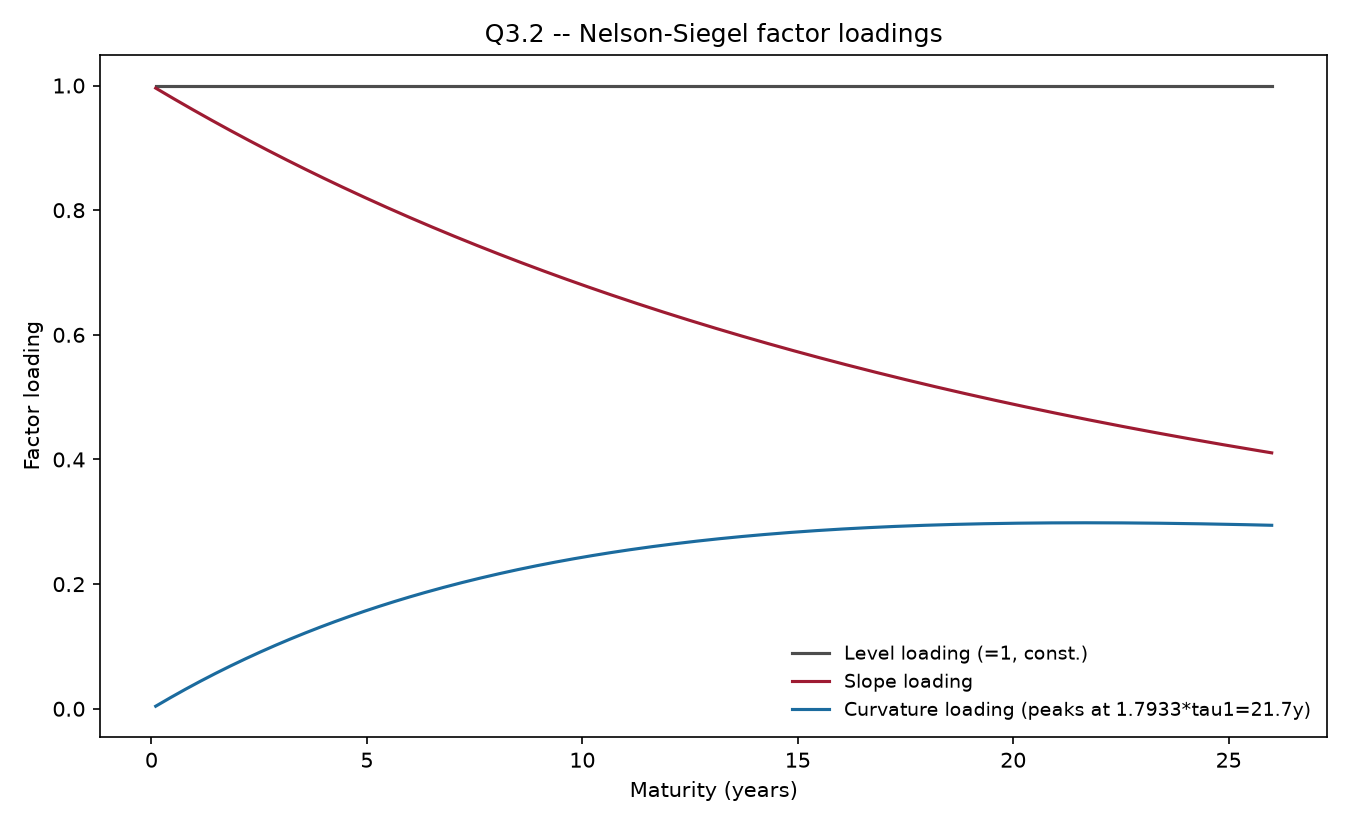
\includegraphics[width=0.78\textwidth]{q3_nss_loadings.png}\\[0.3cm]
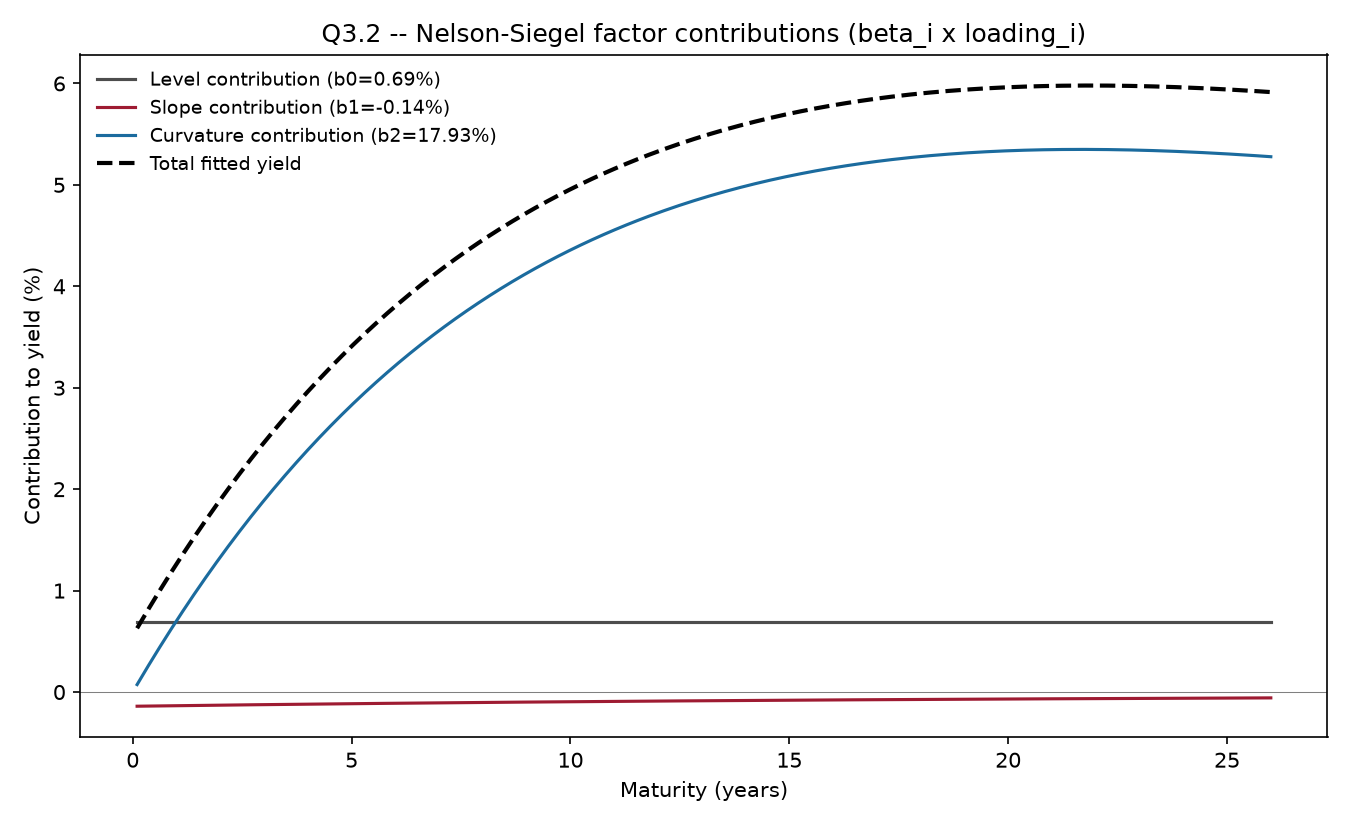
\includegraphics[width=0.78\textwidth]{q3_nss_contributions.png}
\caption{Top: factor loadings. Bottom: factor contributions ($\beta_i \times$ loading$_i$).}
\end{figure}

The contribution decomposition reveals a striking feature: the
\textbf{curvature} factor ($\beta_2=17.9\%$) does almost all of the
curve-shaping work, rising smoothly from 0 at $m=0$ to its asymptote around
20 years, while the level contribution is small and essentially flat
($0.695\%$) and the slope contribution is tiny and nearly flat
($-0.140\%$). This is counter-intuitive at first glance --- in textbook
Nelson-Siegel intuition, ``level'' should dominate a curve of this overall
magnitude --- but it is a direct, mechanical consequence of $\tau_1$ being
large ($12.08$ years) relative to our 26-year maturity range: the curvature
loading function $\left[\frac{1-e^{-m/\tau_1}}{m/\tau_1}-e^{-m/\tau_1}\right]$
simply has not decayed back to zero by $m=26$, so it is statistically
\emph{behaving like} a second, slowly-varying level/slope factor over the
range of our data, and the OLS step naturally loads most of the explanatory
power onto it rather than onto $\beta_0$ precisely because $\beta_0$'s
loading is flat and uninformative about curve \emph{shape}, whereas the
curvature loading can trace the whole concave shape on its own.

Economically, this echoes Deutsche Bank's own Exhibit 3 three-factor model
description: a persistent, long-horizon ``long-rate''/level-type factor
that evolves slowly is naturally captured by a Nelson-Siegel factor whose
decay parameter is large relative to the fitting window, rather than by the
model's nominal level factor, which by construction carries no shape
information at all. In other words, when the sample's maturity range is not
much longer than $\tau_1$, Nelson-Siegel's ``curvature'' factor and a
slow-moving macro ``long rate'' factor become difficult to tell apart ---
exactly the level/curvature identifiability issue we had already flagged
during estimation (Q3.1).

%--------------------------------------------------------------------
\question{Q4 --- Answer summary}

\begin{center}
\fbox{\parbox{0.94\textwidth}{\small
\noindent\textbf{Q4.1.} A $+50$bps bump of the 10Y knot with the natural spline
re-fitted raises the 10Y zero yield by exactly $50$bps and leaves the other
four knots unchanged, but the shock is \emph{not} local: the curve ripples
($+22.1$bps at 7Y, $-8.4$bps at 17Y, $-11.5$bps at 26Y).\\[3pt]
\textbf{Q4.2.} $\text{KRD}_{10Y}=2.21$ years $(\Delta P=-\$10{,}813.14$, i.e.\
$-1.08\%$ of NAV; $\text{DV01}=\$221.0$ central, $\$216.3$ one-sided).\\[3pt]
\textbf{Q4.3.} The 52 individual zero-yield KRDs sum to $7.981$ years, exactly
the portfolio's effective duration; the aggregated key-rate profile is
$0.37/1.54/2.21/0.81/3.06$ years at 2/5/10/15/20Y.
}}
\end{center}

%--------------------------------------------------------------------
\question{Q4.1 --- Shocking the 10Y key rate}

\textbf{Methodology.} The Q2.1 curve is a natural cubic spline through the
bootstrapped zero yields at the knots 2, 5, 10, 15 and 20y, which are exactly
the assignment's key rates. We therefore implement ``shock the 10-year rate by
50bps'' literally on that model: we add $+50$bps to the 10Y knot value,
\emph{re-fit} the natural spline, and define the curve shock as
$$\Delta y(t) = S_{\text{bumped}}(t) - S_{\text{base}}(t), \qquad t = 0.5, 1.0, \dots, 26\text{y}.$$
Because spline interpolation is linear in the knot values, $\Delta y(t)$ does
not depend on the level of the curve, and the five key-rate shocks sum
\emph{exactly} to a $+50$bps parallel shift at every maturity (verified in the
code). For comparison, we also run the textbook Ho (1992) triangular
(``tent'') shock: full size at its own knot, decaying linearly to zero at the
adjacent knots, and held flat beyond the outer knots.

\begin{figure}[h]
\centering
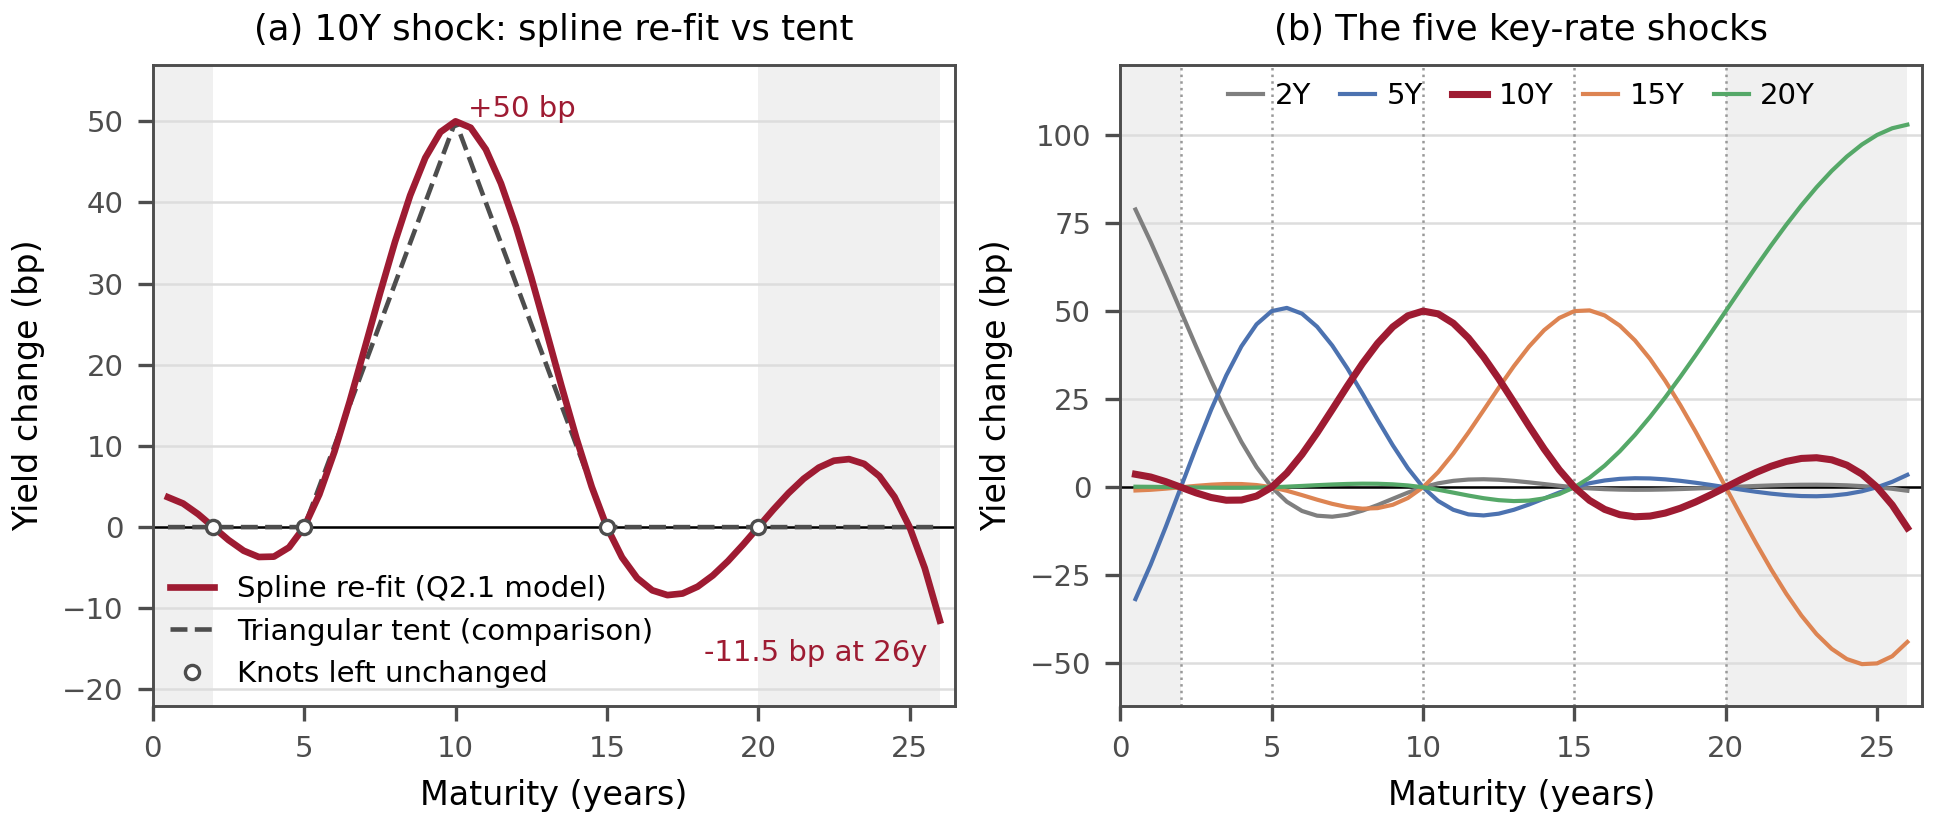
\includegraphics[width=\textwidth]{q4_1_shock_10y.png}
\caption{Left: the curve shock $\Delta y(t)$ from re-fitting the spline (red)
vs.\ the triangular tent (dashed); hollow markers are the four knots left
unchanged. Right: the five spline key-rate shocks. Shaded areas: extrapolated
maturities ($<2$y, $>20$y).}
\end{figure}

\textbf{Impact on the curve.} The shock is $+50$bps at 10Y and, by
construction, zero at the other knots (2, 5, 15, 20y). However, unlike the
tent, the spline response is \textbf{not local}:
\begin{itemize}[nosep]
\item Between 5Y and 15Y it is \emph{wider} than the tent: $+22.1$bps at 7y
and $+37.0$bps at 12y, versus $+20$ and $+30$bps for the linear ramp.
\item Outside $[5,15]$y the cubic \emph{ripples} with alternating signs:
about $-3$ to $-4$bps between 3 and 4y, $-8.4$bps at 17y, and $+8.4$bps at 23y.
\item In the \textbf{extrapolated} region beyond 20y the spline continues the
last cubic polynomial --- the \texttt{CubicSpline} implementation extends the
end cubic, it does not hold the curve flat --- so the ripple grows to
$-11.5$bps at 26y. (A flat extension would put the 26Y yield at $5.95\%$
instead of $6.35\%$ and would set this last contribution to zero; we keep the
model-consistent extension and quantify the sensitivity in Q4.3.) The right
panel shows that this effect is much stronger for the outer knots: a 20Y bump
moves the 26y yield by about $+103$bps, a 15Y bump moves it by about
$-44$bps, and a 2Y bump moves the 0.5y yield by $+79$bps.
\end{itemize}

\begin{table}[h]
\centering
\footnotesize
\begin{tabular}{l *{11}{r}}
\toprule
Maturity (y) & 2 & 3 & 5 & 7 & 10 & 12 & 15 & 17 & 20 & 23 & 26 \\
\midrule
$\Delta y$, spline re-fit (bps) & 0.0 & $-2.9$ & 0.0 & $+22.1$ & $+50.0$ & $+37.0$ & 0.0 & $-8.4$ & 0.0 & $+8.4$ & $-11.5$ \\
$\Delta y$, tent (bps)          & 0.0 & 0.0 & 0.0 & $+20.0$ & $+50.0$ & $+30.0$ & 0.0 & 0.0 & 0.0 & 0.0 & 0.0 \\
\bottomrule
\end{tabular}
\caption{The $+50$bps 10Y shock at selected maturities: global spline re-fit
vs.\ the local triangular tent. $\Delta y$ is zero at 5Y and 15Y because the
tent is a straight line between the knots; it is zero at 2, 5, 15 and 20Y for
the re-fit because those knots are not moved.}
\end{table}

In short, a key-rate shock is only as local as the curve model it is applied
to. The tent is local by design, while a cubic spline spreads a single-node
shock across the whole curve, most strongly where the curve is extrapolated
rather than interpolated.

%--------------------------------------------------------------------
\question{Q4.2 --- Portfolio KRD to the 10Y shock}

\textbf{Portfolio construction (assumption).} ``Equally invested'' is read as
an equal \emph{dollar market value}: \$1,000,000/52 $\approx$ \$19{,}230.77
in each bond, i.e.\ a face amount of
$(\text{dollar amount}/\text{price})\times 100$ per bond. The alternative
reading, an equal \emph{face} amount (\$19{,}230.77 of face in each bond),
would give a \$1.19m market value and $\text{KRD}_{10Y}=2.31$y: equal face
overweights the cheap short bonds and underweights the expensive long ones,
so it raises duration. We use equal market value, the standard reading of
``equally invested'', and report the alternative in the robustness table.

\textbf{Approach.}
\begin{enumerate}[nosep]
\item Build the $52\times52$ cash-flow matrix (semi-annual coupons plus
principal) and aggregate it into the portfolio cash flow at each semi-annual
date.
\item \emph{Base valuation} uses the Q1.1 bootstrapped zero curve (BEY,
semi-annual compounding). It reprices every bond exactly, so the base NAV is
exactly \$1,000,000. Pricing off the spline itself would give
\$1,002,389, and the \$2,389 gap (the Q2.2 fitting residual) would
contaminate the risk measure.
\item \emph{Shocked valuation}: add the spline-implied $\Delta y(t)$ from Q4.1
to the bootstrapped yields and reprice. The shape of the shock therefore
comes from the Q2.1 model, while the base level matches market prices.
\item Report the result as (i) the dollar P\&L of the $+50$bps shock;
(ii) the KRD in years, using a central difference to strip out convexity,
$\text{KRD}_k = -\dfrac{P(+h)-P(-h)}{2\,P_0\,h}$ with $h=50$bps; and
(iii) the DV01 (\$ per 1bp), which is the quantity used to size hedges.
\end{enumerate}

\textbf{Result.}
$$\boxed{\Delta P_{10Y} = \$989{,}186.86 - \$1{,}000{,}000.00 = -\$10{,}813.14
\;(-1.08\%\text{ of NAV}), \qquad \text{KRD}_{10Y} = 2.21\text{ years},
\qquad \text{DV01}_{10Y} = \$221.0}$$
The sign is as expected: a long bond portfolio loses value when yields rise.
The \$221.0 is a \emph{central}-difference DV01,
$\text{DV01}=-(P(+h)-P(-h))/2\times10^{-4}$; the \emph{one-sided} $+50$bps
P\&L implies \$216.26 per bp, so $\Delta P\neq-50\times\text{DV01}$. The
\$4.8 per bp gap is the convexity term, which a 50bp move is large enough to
reveal; we report the central figure because it is the one used to size the
hedge in Q4.3.

\textbf{What actually moves the number (robustness).} The KRD is essentially
invariant to the pricing engine and materially sensitive to the \emph{shock
design}, which is where most of the dispersion between reasonable
implementations comes from:

\begin{center}
\small
\begin{tabular}{lrr}
\toprule
Variant & $\Delta P$ for $+50$bps & $\text{KRD}_{10Y}$ (yrs) \\
\midrule
Spline re-fit, bootstrapped base (\textbf{reported}) & $-\$10{,}813$ & 2.210 \\
Spline re-fit, spline-priced base & $-\$10{,}954$ & 2.234 \\
Triangular tent, bootstrapped base & $-\$10{,}123$ & 2.061 \\
Triangular tent, spline-priced base & $-\$10{,}232$ & 2.078 \\
Single-point 10Y bump (10Y zero yield only) & $-\$1{,}169$ & 0.240 \\
Equal-face portfolio, bootstrapped base & $-\$13{,}445$ & 2.307 \\
\bottomrule
\end{tabular}
\end{center}

Every defensible convention puts the 10Y exposure between $2.0$ and $2.4$
years; the spread is methodological, not arithmetic. We report $2.21$y
because (i) Q4.1 asks for the impact on the curve \emph{estimated in Q2.1},
which is the re-fitted spline, and (ii) pricing the base off the bootstrap
keeps $P_0$ exactly at the $\$1$m actually invested, so the $-\$2{,}389$ Q2.2
fitting residual cannot leak into the risk measure. The $0.24$y row shows the
opposite extreme: applying the shock to the single 10Y zero yield only
measures the partial duration of one cash-flow date, not a key-rate duration.

%--------------------------------------------------------------------
\question{Q4.3 --- Full key-rate duration profile}

\textbf{(a) Each of the 52 zero-coupon yields individually (the literal
reading).} ``All maturities'' is read as applying the same $+50$bps shock to
each semi-annual zero yield (0.5y to 26y) \emph{on its own}, leaving the other
51 unchanged. This version needs no curve model: only the discount factor of
that single date moves, so to first order the KRD at date $t$ is
$t\times\text{PV}(\text{CF}_t)/\text{NAV}$ (i.e.\
$[t/(1+y_t/2)]\times\text{PV}(\text{CF}_t)/\text{NAV}$ in BEY terms).

\begin{figure}[h]
\centering
\includegraphics[width=0.8\textwidth]{q4_3_krd_by_maturity.png}
\caption{KRD to each individual zero-coupon yield ($+50$bps). The 52 bars sum
to 7.981 years, the portfolio's effective duration.}
\end{figure}

\textbf{Additivity check.} The 52 KRDs sum to $7.9809$ years, exactly the
effective duration of a $\pm50$bps parallel shift: a parallel shift is the
sum of the 52 single-date shocks, so this check needs no curve model and is
free of cross terms.

\textbf{Shape of the profile.} The exposure at date $t$ is roughly
$t\times$(PV of the portfolio cash flow at $t$)/NAV. It rises with $t$ to a
peak of $0.24$y at 10y, then \emph{drops abruptly} at 10.5y. Bonds maturing
from Feb-2014 onwards carry high coupons (5.25--13.25\%) and mostly trade far
above par (up to 174), so an equal \emph{dollar} allocation buys less face
--- hence less principal --- at those dates. Beyond 10.5y the exposure
declines slowly as discounting erodes the PV of distant cash flows.

\textbf{(b) The five key rates (aggregated view).} We apply the same $+50$bps
re-fit shock to each knot in turn.

\begin{table}[h]
\centering
\small
\begin{tabular}{r rrr r rr}
\toprule
 & \multicolumn{3}{c}{Spline re-fit (Q2.1 model)} & & \multicolumn{2}{c}{Tent (comparison)} \\
\cmidrule{2-4}\cmidrule{6-7}
Key rate & P\&L (\$) & KRD (yrs) & DV01 (\$) & & P\&L (\$) & KRD (yrs) \\
\midrule
2Y  & $-1{,}820$  & 0.367 & 36.7  & & $-2{,}640$  & 0.531 \\
5Y  & $-7{,}594$  & 1.541 & 154.1 & & $-7{,}156$  & 1.446 \\
10Y & $-10{,}813$ & 2.210 & 221.0 & & $-10{,}123$ & 2.061 \\
15Y & $-3{,}496$  & 0.810 & 81.0  & & $-8{,}236$  & 1.690 \\
20Y & $-13{,}980$ & 3.064 & 306.4 & & $-10{,}717$ & 2.252 \\
\midrule
Sum & $-37{,}704$ & 7.992 & 799.2 & & $-38{,}872$ & 7.979 \\
\bottomrule
\end{tabular}
\caption{Key-rate exposures of the \$1M equally-weighted portfolio
($+50$bps shock at each knot). The parallel-shift effective duration is
7.981 years. KRD and DV01 are central differences; the P\&L column is
one-sided, so P\&L $\neq -50\times$DV01.}
\end{table}

\begin{figure}[h]
\centering
\includegraphics[width=0.72\textwidth]{q4_3_krd_profile.png}
\caption{Key-rate duration profile (years): spline re-fit vs.\ triangular tent.}
\end{figure}

\textbf{Consistency check.} Both families of shocks sum to a parallel shift,
so the KRDs should add up to the effective duration. They do: 7.992y (spline)
and 7.979y (tent), versus 7.981y for a $\pm50$bps parallel shift. Summing the
\emph{one-sided} dollar P\&Ls gives $-\$37{,}704$ versus $-\$38{,}594$ for the
parallel shock. The gap comes from convexity and cross terms, which are
largest for the spline because its extrapolated shocks reach about 100bps.
This is why we report central-difference KRDs.

\textbf{Robustness: the 15Y/20Y split is an extrapolation effect.} The Q2.1
spline is pinned by data only up to 20Y; beyond that, the end cubic amplifies
the effect of a 50bps bump at 20Y to $+103$bps at 26Y, and the effect of a
50bps bump at 15Y to $-50$bps at 24.5Y. That is what moves duration between
the two buckets:

\begin{center}
\small
\begin{tabular}{lrrrrrr}
\toprule
 & 2Y & 5Y & 10Y & 15Y & 20Y & Sum \\
\midrule
End cubic (reported)  & 0.367 & 1.541 & 2.210 & 0.810 & 3.064 & 7.992 \\
Held flat beyond 20Y  & 0.180 & 1.619 & 2.109 & 1.850 & 0.652 & 6.411 \\
\bottomrule
\end{tabular}
\end{center}

Holding the curve flat would move the split to 1.85y (15Y) and 0.65y (20Y),
but the five KRDs would then sum to 6.41y instead of the portfolio's 7.98y
effective duration, because the shocks would no longer sum to a parallel
shift: the cash flows beyond 20Y, about 1.57y of duration, would carry no
key-rate exposure at all. We keep the model-consistent extension --- it is
the only one under which the key-rate decomposition is complete --- and
present the 15Y/20Y split as model risk rather than as a tradable exposure.

\textbf{Interpretation.}
\begin{itemize}[nosep]
\item All exposures are positive durations (negative P\&L), as expected for
a long-only portfolio.
\item With the tent, the profile is smooth (0.53 / 1.45 / 2.06 / 1.69 /
2.25y) and follows the cash-flow intuition; the 20Y bucket is the largest
because it also absorbs every maturity from 20 to 26y.
\item With the spline re-fit, the ripples of Q4.1 redistribute risk. The 2Y
KRD falls to 0.37y (vs.\ 0.53y): the 2Y bump pushes 5--10y yields \emph{down}
by up to 8.4bps, worth $+\$1{,}063$ on the 5--10y cash flows, which more than
offsets the extra $-\$219$ caused by its larger short-end shock ($+79$bps at
0.5y vs.\ $+50$bps for the tent). The 15Y/20Y split moves as explained above.
The total is unchanged, which is the point.
\item \textbf{Practical implication.} The choice of curve model is itself a
source of hedging risk. A hedge sized on spline KRDs would put far more
weight on 20Y and far less on 15Y than a hedge sized on tent KRDs, even
though both imply the same total duration.
\end{itemize}

\textbf{Illustrative KRD hedge (beyond the question).} Neutralising the five
spline key-rate DV01s with the five bonds maturing exactly at the key dates
requires short \$93.6k (Aug-2005), short \$199.5k (Aug-2008), short \$211.5k
(Aug-2013), \emph{long} \$19.4k (Aug-2018) and short \$445.6k (Aug-2023), for
a hedge market value of $-\$968$k (the funding leg is not modelled). The
$+50$bps parallel P\&L falls from $-\$38{,}594$ to $+\$57$; the individual
key-rate residuals are at most \$606 (20Y), from second-order convexity.

\newpage
%Paolo
%====================================================================
\section{Part II --- Python Labs: US Treasury Yield Curve Reaction to Trump Tariff Threats}

\subsection*{Data, event set and conventions}

\textbf{Data.} Daily US Treasury constant-maturity yields for ten maturities,
from 3 months to 30 years (FRED series \texttt{DGS3MO} to \texttt{DGS30}),
downloaded with the course helper \texttt{fred.py}. The sample used in Q1 runs from 2 January 2015 to 1 August 2025, i.e.\
2{,}647 trading days. Yields are in percent; all results are reported in basis
points (bp).

\textbf{Code.} A single run of \nolinkurl{ga_project/06_event_study.py}
reproduces every number, table and figure of this part (output files are
prefixed \texttt{pl\_}). The original course notebook is in
\nolinkurl{ga_project/python_labs/}.

\textbf{Event set.} The notebook's \texttt{trump\_actions} and
\texttt{country\_responses} dictionaries contain 75 events: 36 Trump actions
and 39 foreign responses (Python silently keeps only the last entry of each
duplicated date key, so two listed events are lost). Mapping the events to
trading days:
\begin{itemize}[leftmargin=1.2em,nosep]
\item 8 events fall after 1 August 2025, when the FRED download ends, and are
dropped;
\item 16 events fall on a weekend or a market holiday and are moved to the
next trading day (e.g.\ the events of Saturday 5 and Sunday 6 April 2025 both
map to Monday 7 April);
\item 9 trading days carry two events. On 8 of them a Trump action and a
foreign response share the same day (e.g.\ 2018-07-06, 2019-08-23,
2025-03-04); on the ninth, the 4 July 2025 holiday collapses onto the
7 July action.
\end{itemize}
The remaining 67 events therefore correspond to \textbf{58 distinct event
days}, each counted once. All 58 have a full pre-event window; 51 have a full
30-day post-event window, because the last events of the sample are followed
by fewer than 30 trading days of data.

\textbf{Methodology (as required by the assignment).} Let $t_1,\dots,t_N$ be
the event days and $y_t$ a yield, or one of the three curve factors
\[
\text{level}=y_{10},\qquad
\text{slope}=y_{10}-y_{2},\qquad
\text{curvature}=2\,y_{5}-y_{2}-y_{10},
\]
where $y_m$ is the $m$-year yield. For each horizon $k=-30,\dots,+30$ trading
days, the abnormal change is
\[
\mathrm{AC}(k)
=\frac{1}{N}\sum_{i=1}^{N}\bigl(y_{t_i+k}-y_{t_i}\bigr)
-\frac{1}{|\mathcal{B}_k|}\sum_{s\in\mathcal{B}_k}\bigl(y_{s+k}-y_{s}\bigr),
\]
where $\mathcal{B}_k$ is the set of non-event days $s$ such that both $s$ and
$s+k$ lie more than 30 trading days away from every event. The first term is
the average change around the events; the second is the ``normal'' change
over the same horizon.

\textbf{Reading the results.} Because $\mathrm{AC}(k)$ is measured relative
to the event day, a \emph{positive} value at $k<0$ means that yields were
\emph{higher} before the event, i.e.\ they \emph{fell} into it. To avoid this
sign trap, every table reports three windows as the abnormal change in yield
\emph{over the window} (positive $=$ yields rose):
\begin{itemize}[leftmargin=1.2em,nosep]
\item \textbf{pre-event} $[-30,0]$: $\;y_{t}-y_{t-30}$, i.e.\ $-\mathrm{AC}(-30)$;
\item \textbf{announcement} $[-1,+1]$: $\;y_{t+1}-y_{t-1}$, i.e.\ $\mathrm{AC}(+1)-\mathrm{AC}(-1)$;
\item \textbf{post-event} $[0,+30]$: $\;y_{t+30}-y_{t}$, i.e.\ $\mathrm{AC}(+30)$.
\end{itemize}

\textbf{Assumptions.}
\begin{itemize}[leftmargin=1.2em,nosep]
\item[(A1)] Business days are the trading days present in the FRED data;
weekend and holiday events move to the next trading day.
\item[(A2)] The ``reaction of targeted countries'' (Q1.3) is measured on the
\emph{US} curve on the dates of the foreign responses, since only US yields
are provided.
\item[(A3)] Q1 uses the notebook's event list, sample and baseline unchanged;
all corrections are made in Q2.1.
\item[(A4)] To judge magnitudes we also report the \emph{raw} average change
around the events with its cross-sectional standard error (s.e.). These
s.e.\ treat events as independent; since windows overlap, they overstate
precision and are only a first indication.
\end{itemize}

%--------------------------------------------------------------------
\question{Q1.1 --- Market reaction to Trump's announcements and actions}

\begin{figure}[!htbp]
\centering
\includegraphics[width=\textwidth]{pl_q11_q13_paths.png}
\caption{Abnormal change relative to the event day (bp), assignment
methodology. Left: Trump actions (Q1.1). Right: foreign responses (Q1.3). A
line falling from left to right means that yields fell through the window.}
\label{fig:q11}
\end{figure}

\begin{table}[!htbp]
\centering
\small
\begin{tabular}{lrrrrr}
\toprule
 & 3M & 2Y & 5Y & 10Y & 30Y \\
\midrule
\multicolumn{6}{l}{\emph{Panel A. Abnormal change (assignment methodology), bp}} \\
\addlinespace[2pt]
Pre-event $[-30,0]$     & $-6.4$ & $-10.2$ & $-11.6$ & $-11.1$ & $-9.5$ \\
Announcement $[-1,+1]$  & $-0.5$ & $-1.6$  & $-0.8$  & $-0.2$  & $+0.6$ \\
Post-event $[0,+30]$    & $-7.1$ & $-14.0$ & $-13.6$ & $-9.5$  & $-4.5$ \\
\addlinespace
\multicolumn{6}{l}{\emph{Panel B. Post-event window decomposed: abnormal $=$ raw $-$ baseline, bp}} \\
\addlinespace[2pt]
Raw change around events & $+1.4$ & $-6.8$ & $-7.4$ & $-3.5$ & $+1.0$ \\
\quad (s.e.)             & $(3.1)$ & $(5.3)$ & $(5.5)$ & $(5.2)$ & $(4.8)$ \\
Non-event baseline       & $+8.5$ & $+7.2$ & $+6.2$ & $+5.9$ & $+5.5$ \\
\bottomrule
\end{tabular}
\caption{Trump actions: 32 event days in the pre-event and announcement
windows, 28 in the post-event window. Panel B may not add up exactly because
of rounding.}
\label{tab:q11}
\end{table}

\textbf{Discussion.}
\begin{itemize}[leftmargin=1.2em,nosep]
\item \textbf{No announcement effect.} Over $[-1,+1]$ the curve barely moves:
$-1.6$\,bp on the 2Y and $-0.2$\,bp on the 10Y, against raw s.e.\ of about
1.2--1.5\,bp. Nothing is distinguishable from zero.
\item \textbf{Large abnormal declines on both sides of the event.} Taken at
face value, Panel~A says that yields fall by 10--12\,bp (2Y to 10Y) in the
30 days \emph{before} the events and by a further 5--14\,bp \emph{after}
them, most at the front end. The textbook reading is a negative growth shock:
flight to quality into Treasuries and higher odds of Fed cuts, which lowers
the 2Y most.
\item \textbf{But most of it is the baseline.} Panel~B shows that the raw
change after the events is small and statistically zero: $-3.5$\,bp on the
10Y (s.e.\ 5.2) and $+1.0$\,bp on the 30Y. The ``abnormal'' declines come
mainly from subtracting a non-event baseline of $+5.5$ to $+8.5$\,bp per 30 days.
That baseline is computed on days far from any event, i.e.\ mostly 2015--16
and 2020--24, a period dominated by the 2022--23 hiking cycle, when yields
were rising.
\item \textbf{The shape confirms it.} A reaction to news would be a jump
around day 0; Figure~\ref{fig:q11} instead shows a smooth 60-day ramp that
starts a month before the announcements. This is the signature of a trend
difference between event periods (2018--19, 2025) and the baseline period,
not of a tariff effect.
\end{itemize}
\textbf{Answer.} With the required methodology, Treasury yields appear to fall
around Trump's tariff actions (about $-10$ to $-14$\,bp at the 2Y--5Y over
30 days). However, there is no announcement effect, and the post-event decline
is driven by the choice of baseline rather than by the events. Q2.1 tests this
directly.

%--------------------------------------------------------------------
\question{Q1.2 --- Level, slope and curvature}

\begin{figure}[!htbp]
\centering
\includegraphics[width=\textwidth]{pl_q12_lsc.png}
\caption{Abnormal change of level, slope and curvature (bp): Trump actions
(red) vs.\ all events (dashed).}
\end{figure}

\begin{table}[!htbp]
\centering
\small
\begin{tabular}{lrrrcrrr}
\toprule
 & \multicolumn{3}{c}{Trump actions} & & \multicolumn{3}{c}{All events} \\
\cmidrule{2-4}\cmidrule{6-8}
Abnormal change, bp & Level & Slope & Curv. & & Level & Slope & Curv. \\
\midrule
Pre-event $[-30,0]$    & $-11.1$ & $-1.0$ & $-1.8$ & & $-11.5$ & $-1.3$ & $-2.9$ \\
Announcement $[-1,+1]$ & $-0.2$  & $+1.4$ & $+0.1$ & & $-0.2$  & $+1.3$ & $-0.1$ \\
Post-event $[0,+30]$   & $-9.5$  & $+4.5$ & $-3.7$ & & $-7.7$  & $+2.0$ & $-4.0$ \\
\addlinespace
\emph{Raw post-event change (s.e.)} & $-3.5$ & $+3.3$ & $-4.4$ & & & & \\
 & $(5.2)$ & $(1.9)$ & $(1.2)$ & & & & \\
\bottomrule
\end{tabular}
\caption{Level ($=$ 10Y), slope ($=$ 10Y $-$ 2Y) and curvature
($=2\times$5Y $-$ 2Y $-$ 10Y).}
\label{tab:q12}
\end{table}

\textbf{Discussion.}
\begin{itemize}[leftmargin=1.2em,nosep]
\item \textbf{Level} reproduces Q1.1 by construction, since it is the 10Y.
The level effect is therefore subject to the same baseline caveat: raw
$-3.5$\,bp, s.e.\ 5.2. A level factor based on all maturities (first
principal component) is used in Q2.1.
\item \textbf{Slope.} After Trump actions the curve \emph{steepens}: $+1.4$\,bp
over $[-1,+1]$ and $+4.5$\,bp over 30 days, while the level falls. This is a
\emph{bull steepening}: the front end, anchored to expected policy rates,
rallies more than the 10Y, which also carries tariff-driven inflation risk and
a term premium. Unlike the level, the slope is barely affected by the
baseline ($-1.3$\,bp): the raw steepening is $+3.3$\,bp (s.e.\ 1.9). It is
partly offset by a flattening in the run-up ($-1.0$\,bp abnormal), so the
evidence is weak but this is the most event-like pattern in Q1.
\item \textbf{Curvature} falls after the events ($-3.7$\,bp): the 5Y belly
rallies more than the average of the 2Y and 10Y wings. This would be
consistent with cuts priced over the next 2--5 years. However, curvature
also falls \emph{before} the events (raw $-2.5$\,bp) and after foreign
responses (raw $-4.5$\,bp). That points to a downward trend in curvature
during the event periods rather than a reaction to tariff news.
\item \textbf{All events vs.\ Trump actions.} Level and slope effects are
weaker when foreign responses are included (post-event slope $+2.0$ vs.\
$+4.5$\,bp), while curvature is unchanged, consistent with the trend
interpretation.
\end{itemize}

%--------------------------------------------------------------------
\question{Q1.3 --- Market reaction to the targeted countries' responses}

\begin{table}[!htbp]
\centering
\small
\begin{tabular}{lrrrrrrr}
\toprule
 & 3M & 2Y & 5Y & 10Y & 30Y & Slope & Curv. \\
\midrule
\multicolumn{8}{l}{\emph{Panel A. Abnormal change (assignment methodology), bp}} \\
\addlinespace[2pt]
Pre-event $[-30,0]$    & $-2.6$ & $-11.8$ & $-15.3$ & $-14.3$ & $-10.9$ & $-2.4$ & $-4.4$ \\
Announcement $[-1,+1]$ & $+0.1$ & $-1.1$  & $-0.2$  & $+0.7$  & $+0.9$  & $+1.8$ & $0.0$ \\
Post-event $[0,+30]$   & $-3.2$ & $-2.7$  & $-3.7$  & $-0.6$  & $+1.8$  & $+2.1$ & $-4.1$ \\
\addlinespace
\multicolumn{8}{l}{\emph{Panel B. Raw post-event change, bp}} \\
\addlinespace[2pt]
Raw change    & $+4.2$ & $+4.1$ & $+2.2$ & $+4.8$ & $+6.5$ & $+0.6$ & $-4.5$ \\
\quad (s.e.)  & $(2.3)$ & $(3.7)$ & $(3.8)$ & $(3.8)$ & $(3.7)$ & $(2.2)$ & $(1.0)$ \\
\bottomrule
\end{tabular}
\caption{Foreign responses: 34 event days in the pre-event window, 33 in the
announcement window, 31 in the post-event window.}
\label{tab:q13}
\end{table}

\textbf{Discussion.}
\begin{itemize}[leftmargin=1.2em,nosep]
\item \textbf{Before the responses} yields fall by 11--15\,bp (2Y to 30Y).
This is largely mechanical: a response typically comes a few days after the
US measure it answers, so its pre-event window contains the US action itself.
In eight cases the two fall on the same trading day.
\item \textbf{At the announcement} nothing moves beyond noise (at most
$+0.9$\,bp on yields, $+1.8$\,bp on the slope).
\item \textbf{After the responses}, the abnormal change is close to zero
(10Y $-0.6$\,bp). In raw terms, however, yields \emph{rise} by 2--7\,bp, the
30Y the most ($+6.5$\,bp, s.e.\ 3.7). These rises are absorbed by the rising
baseline. So ``no abnormal reaction'' means that yields behaved like in an
average non-event month, not that they were flat.
\item \textbf{Economic reading.} Retaliation has two opposite effects on US
yields. It hurts US exporters, which is growth-negative and lowers yields. It
also raises import prices and threatens foreign demand for Treasuries, which
pushes up inflation expectations and the term premium. The mild rise of the
long end relative to the front end (slope $+1.8$\,bp at the announcement)
suggests that the second channel slightly dominates. The evidence, however,
is weak and concentrated in 2025 (Q1.4).
\end{itemize}

%--------------------------------------------------------------------
\question{Q1.4 --- First vs.\ second mandate}

\begin{figure}[!htbp]
\centering
\includegraphics[width=\textwidth]{pl_q14_terms.png}
\caption{Abnormal change by mandate: first term (2017--20, blue) vs.\ second
term (2025, orange). Top: Trump actions. Bottom: foreign responses.}
\end{figure}

\begin{table}[!htbp]
\centering
\footnotesize
\setlength{\tabcolsep}{3.5pt}
\begin{tabular}{lcrrrrcrrrr}
\toprule
 & & \multicolumn{4}{c}{Pre-event $[-30,0]$, bp} & & \multicolumn{4}{c}{Post-event $[0,+30]$, bp} \\
\cmidrule{3-6}\cmidrule{8-11}
Group & $n$ & 2Y & 10Y & 30Y & Slope & & 2Y & 10Y & 30Y & Slope \\
\midrule
\multicolumn{11}{l}{\emph{Abnormal change (assignment methodology)}} \\
Actions, 1st term & 18/18 & $-3.4$  & $-9.7$  & $-12.3$ & $-6.3$ & & $-6.7$  & $-6.2$  & $-4.8$  & $+0.5$ \\
Actions, 2nd term & 14/10 & $-14.7$ & $-9.5$  & $-3.1$  & $+5.2$ & & $-22.4$ & $-11.7$ & $-1.3$  & $+10.7$ \\
Responses, 1st term     & 22/22 & $-4.1$  & $-12.4$ & $-13.1$ & $-8.3$ & & $+1.7$  & $-0.8$  & $-1.6$  & $-2.5$ \\
Responses, 2nd term     & 12/9  & $-21.8$ & $-14.7$ & $-5.1$  & $+7.1$ & & $-8.6$  & $+3.0$  & $+11.6$ & $+11.6$ \\
\addlinespace
\multicolumn{11}{l}{\emph{Raw post-event change (s.e.)}} \\
Actions, 1st term & & & & & & & $-0.7\,(6.7)$ & $-0.7\,(6.8)$ & $+0.8\,(6.1)$ & $0.0\,(2.2)$ \\
Actions, 2nd term & & & & & & & $-17.9\,(7.9)$ & $-8.7\,(8.5)$ & $+1.2\,(8.2)$ & $+9.2\,(3.0)$ \\
Responses, 2nd term     & & & & & & & $-4.1\,(7.8)$ & $+6.0\,(7.4)$ & $+14.1\,(7.4)$ & $+10.1\,(4.5)$ \\
\bottomrule
\end{tabular}
\caption{Yield change by mandate. Actions $=$ Trump actions; $n$ $=$ event
days in the pre-/post-event windows.}
\label{tab:q14}
\end{table}

\textbf{Discussion.} The two mandates look very different, but for a different
reason than Panel~A alone suggests.
\begin{itemize}[leftmargin=1.2em,nosep]
\item \textbf{First term (2018--19): no measurable reaction.} After Trump
actions the abnormal changes suggest a parallel rally of 5--7\,bp. In raw
terms, however, the 2Y, 10Y and 30Y are all within 1\,bp of zero (s.e.\
about 6--7\,bp): the apparent rally is entirely the baseline. The only clear
first-term feature is a \emph{flattening into the events} (abnormal slope
$-6.3$\,bp after actions, $-8.3$\,bp after responses). This matches the
general flattening of the 2018 hiking cycle more than tariff news. Tariffs
were narrower (mainly China, plus steel and aluminium), inflation was low, and
the Fed's reaction function dominated the curve.
\item \textbf{Second term (2025): a steepening.} Here the raw numbers move:
\begin{itemize}[nosep]
\item After Trump actions, the 2Y falls by 18\,bp while the 30Y does not
move, giving a \emph{bull steepening} (slope $+9.2$\,bp, s.e.\ 3.0): the
front end prices Fed cuts against weaker growth.
\item After foreign responses, the 30Y \emph{rises} by 14\,bp (slope
$+10.1$\,bp), a \emph{bear steepening}.
\end{itemize}
The long end no longer acted as a safe haven. Universal tariffs are
inflationary, fiscal concerns were acute (Moody's downgrade in May, the One
Big Beautiful Bill Act in July), and markets questioned foreign demand for
Treasuries during the April ``sell America'' episode. The shock was absorbed
by the term premium rather than by lower long yields.
\item \textbf{Reliability.} The second-term samples are small: 10 and 9 event
days in the post-event window. They are also concentrated between February and
July 2025, so their 30-day windows overlap and represent only a handful of
independent episodes. The s.e.\ above are therefore too small, and the
differences between mandates are indicative only. Q2.1 tests which of them
survive proper inference.
\end{itemize}

\question{Q2.1 --- Limitations, improvements, and how they change Q1}

\subsection*{(a) Limitations of the design}
\begin{enumerate}[leftmargin=1.4em,itemsep=1pt]
\item \textbf{Biased baseline (regime effect).} The ``normal'' change is
estimated on non-event days, which fall mostly in 2015--16 and 2020--24, a
period dominated by the 2022--23 hiking cycle. The 10Y non-event baseline
therefore rises by $+6.5$\,bp per 30 days, while the average 30-day change was
$-3.6$\,bp in 2017--20 and $-5.8$\,bp in 2025 (Table~\ref{tab:drift}).
Subtracting a rising baseline from falling-rate periods mechanically creates a
negative ``abnormal'' change. Q1 shows that this explains most of the
post-event declines (raw vs.\ abnormal changes in Tables~\ref{tab:q11}
and~\ref{tab:q13}).
\item \textbf{Overlapping windows.} Events come in bursts (e.g.\ 14 events
between 2025-02-01 and 2025-04-10). The 30-day windows therefore overlap and
contain each other's events: observations are not independent, and each long
window mixes many news items.
\item \textbf{No valid inference.} The assignment's design produces averages
without a test. The naive standard errors added in Q1 treat overlapping
windows as independent, so they overstate precision. With 61 horizons and
several series, some ``large'' numbers are bound to appear by chance.
\item \textbf{Event-list quality.}
\begin{itemize}[nosep]
\item Two entries are silently lost to duplicated dictionary keys (2025-08-06
and 2025-03-04).
\item Some entries are not shocks: ``no retaliation'' announcements, a status
quo, and a US court ruling listed as a foreign response.
\item Escalations and de-escalations (Phase One deal, delays, exemptions) are
averaged together, so their effects offset each other.
\item Major milestones are missing: the 90-day pause (2025-04-09), the
US--China Geneva agreement (2025-05-12) and the US--EU deal (2025-07-27).
\item Some descriptions are inaccurate (145\% was the US rate on China).
\end{itemize}
\item \textbf{Sample truncation.} The download stops on 2025-08-01: eight
August-2025 events are dropped and late-July windows are cut short.
\item \textbf{Timing.} Several announcements came after the market close
(``Liberation Day'' on 2025-04-02 was announced after 4pm ET) or on weekends,
so day 0 is not always the reaction day (Figure~\ref{fig:lib}).
\item \textbf{Confounding news.} Some event days coincide with FOMC
decisions, and Trump actions and foreign responses share the same trading day
eight times in the notebook list.
\item \textbf{Measurement.} Level $=$ 10Y duplicates Q1.1. Constant-maturity
par yields are used rather than zero rates, and daily closes cannot isolate an
announcement from other news on the same day.
\end{enumerate}

\begin{table}[!htbp]
\centering
\small
\begin{tabular}{lrrrr}
\toprule
Period & 2015--16 & 2017--20 (1st term) & 2021--24 & 2025 (2nd term) \\
\midrule
Mean 30-day 10Y change (bp) & $+3.3$ & $-3.6$ & $+9.7$ & $-5.8$ \\
\bottomrule
\end{tabular}
\caption{Average 30-day change of the 10Y yield by period. The non-event
baseline of the assignment ($+6.5$\,bp) is dominated by the 2021--24 hiking
cycle.}
\label{tab:drift}
\end{table}

\subsection*{(b) Improvements implemented}
All improvements are in \nolinkurl{06_event_study.py}, function
\texttt{part\_q2}.
\begin{enumerate}[leftmargin=1.4em,itemsep=1pt]
\item \textbf{Cleaned and signed event list.}
\begin{itemize}[nosep]
\item Duplicated keys merged and six non-events removed (list in the code).
\item Each event signed as escalation ($+1$) or de-escalation ($-1$).
\item Three missing de-escalation milestones added.
\item Result: 72 events, of which 63 escalations and 9 de-escalations.
\end{itemize}
\item \textbf{Extended sample} to 2025-10-31, so that every event has a full
window.
\item \textbf{Short windows} $[-1,+1]$ and $[0,+5]$ to capture the
announcement effect. The $[-1,+1]$ window also covers after-close
announcements, whose reaction occurs on day $+1$.
\item \textbf{Baseline from the same mandate.} The expected change is the
average change over windows of the same length that start on ordinary days of
the same mandate, i.e.\ days with no event within $\pm1$ day (913 days in the
first term, 127 in the second). Each event is thus compared with a typical
window of its own rate regime, not with a 2015--2025 average.
\item \textbf{Placebo inference.} For each group we draw 5{,}000 sets of
pseudo-event dates from the same pools, keeping the number of events per
mandate. The two-sided $p$-value is the share of placebo averages at least as
extreme as the actual one.
\begin{itemize}[nosep]
\item A stricter pool (no event within $\pm5$ days) leaves only 56 days in
2025. These are unusually calm days, so the placebo distribution becomes too
narrow and the $p$-values too optimistic.
\item With that pool, 6 results lose significance at 5\% and 5 gain it, but
none of the conclusions below changes (\nolinkurl{pl_q2_placebo_sensitivity.csv}).
\end{itemize}
\item \textbf{De-clustering.} The 30-day window uses only the first event of
each cluster (no other event in the previous 5 trading days).
\item \textbf{Robustness.} We exclude events with a same-day foreign response
and events within $\pm1$ day of an FOMC decision, and we replace the 10Y by a
PCA level (first principal component of daily changes). For 2025 we also drop
April, the month of ``Liberation Day'' and of the Treasury basis-trade
deleveraging (Table~\ref{tab:rob25}).
\end{enumerate}

\begin{table}[!htbp]
\centering
\footnotesize
\setlength{\tabcolsep}{3.5pt}
\begin{tabular}{lrrrrrrrrrr}
\toprule
 & \multicolumn{4}{c}{$[-1,+1]$} & \multicolumn{3}{c}{$[0,+5]$} & \multicolumn{2}{c}{$[0,+30]$, cluster heads} & \\
\cmidrule(lr){2-5}\cmidrule(lr){6-8}\cmidrule(lr){9-10}
Group & 2Y & 10Y & 30Y & Slope & 10Y & 30Y & Slope & 2Y & 10Y & $n$ \\
\midrule
Trump escalations    & $+1.2$ & $+1.5$ & $+2.1$ & $+0.3$ & $+1.8$ & $+2.0$ & $+2.0^{*}$ & $+6.6$ & $+6.1$ & 31/18 \\
\quad 1st term       & $-2.3$ & $-2.2$ & $-1.5$ & $+0.1$ & $-0.6$ & $-0.5$ & $-0.4$ & $+7.9$ & $+7.2$ & 16/12 \\
\quad 2nd term       & $+5.1^{**}$ & $+5.5^{**}$ & $+6.0^{**}$ & $+0.4$ & $+4.3$ & $+4.7^{*}$ & $+4.6^{**}$ & $+4.1$ & $+4.1$ & 15/6 \\
\addlinespace
Foreign escalations  & $+1.8$ & $+3.5^{**}$ & $+3.7^{**}$ & $+1.7^{*}$ & $+4.3^{**}$ & $+4.1^{**}$ & $+2.1^{*}$ & $+4.6$ & $+7.7$ & 32/10 \\
\quad 1st term       & $+0.2$ & $+0.4$ & $+0.7$ & $+0.2$ & $+0.6$ & $-0.4$ & $-1.4$ & $+9.5$ & $+7.7$ & 20/7 \\
\quad 2nd term       & $+4.6^{**}$ & $+8.8^{**}$ & $+8.8^{**}$ & $+4.2^{**}$ & $+10.5^{**}$ & $+11.6^{**}$ & $+7.7^{**}$ & $-6.9$ & $+7.6$ & 12/3 \\
\addlinespace
De-escalations (all) & $+7.0^{**}$ & $+6.7^{**}$ & $+5.9^{**}$ & $-0.3$ & $+1.9$ & $+2.9$ & $+2.6$ & $-20.6^{**}$ & $-19.7^{**}$ & 9/4 \\
\bottomrule
\end{tabular}
\caption{Improved design: abnormal change in bp (positive $=$ yields up)
relative to ordinary windows of the same mandate, extended sample, cleaned
events. Placebo $p$-values: $^{*}p<0.10$, $^{**}p<0.05$. $n$ $=$ events in
the short / 30-day windows.}
\label{tab:improved}
\end{table}

\begin{figure}[!htbp]
\centering
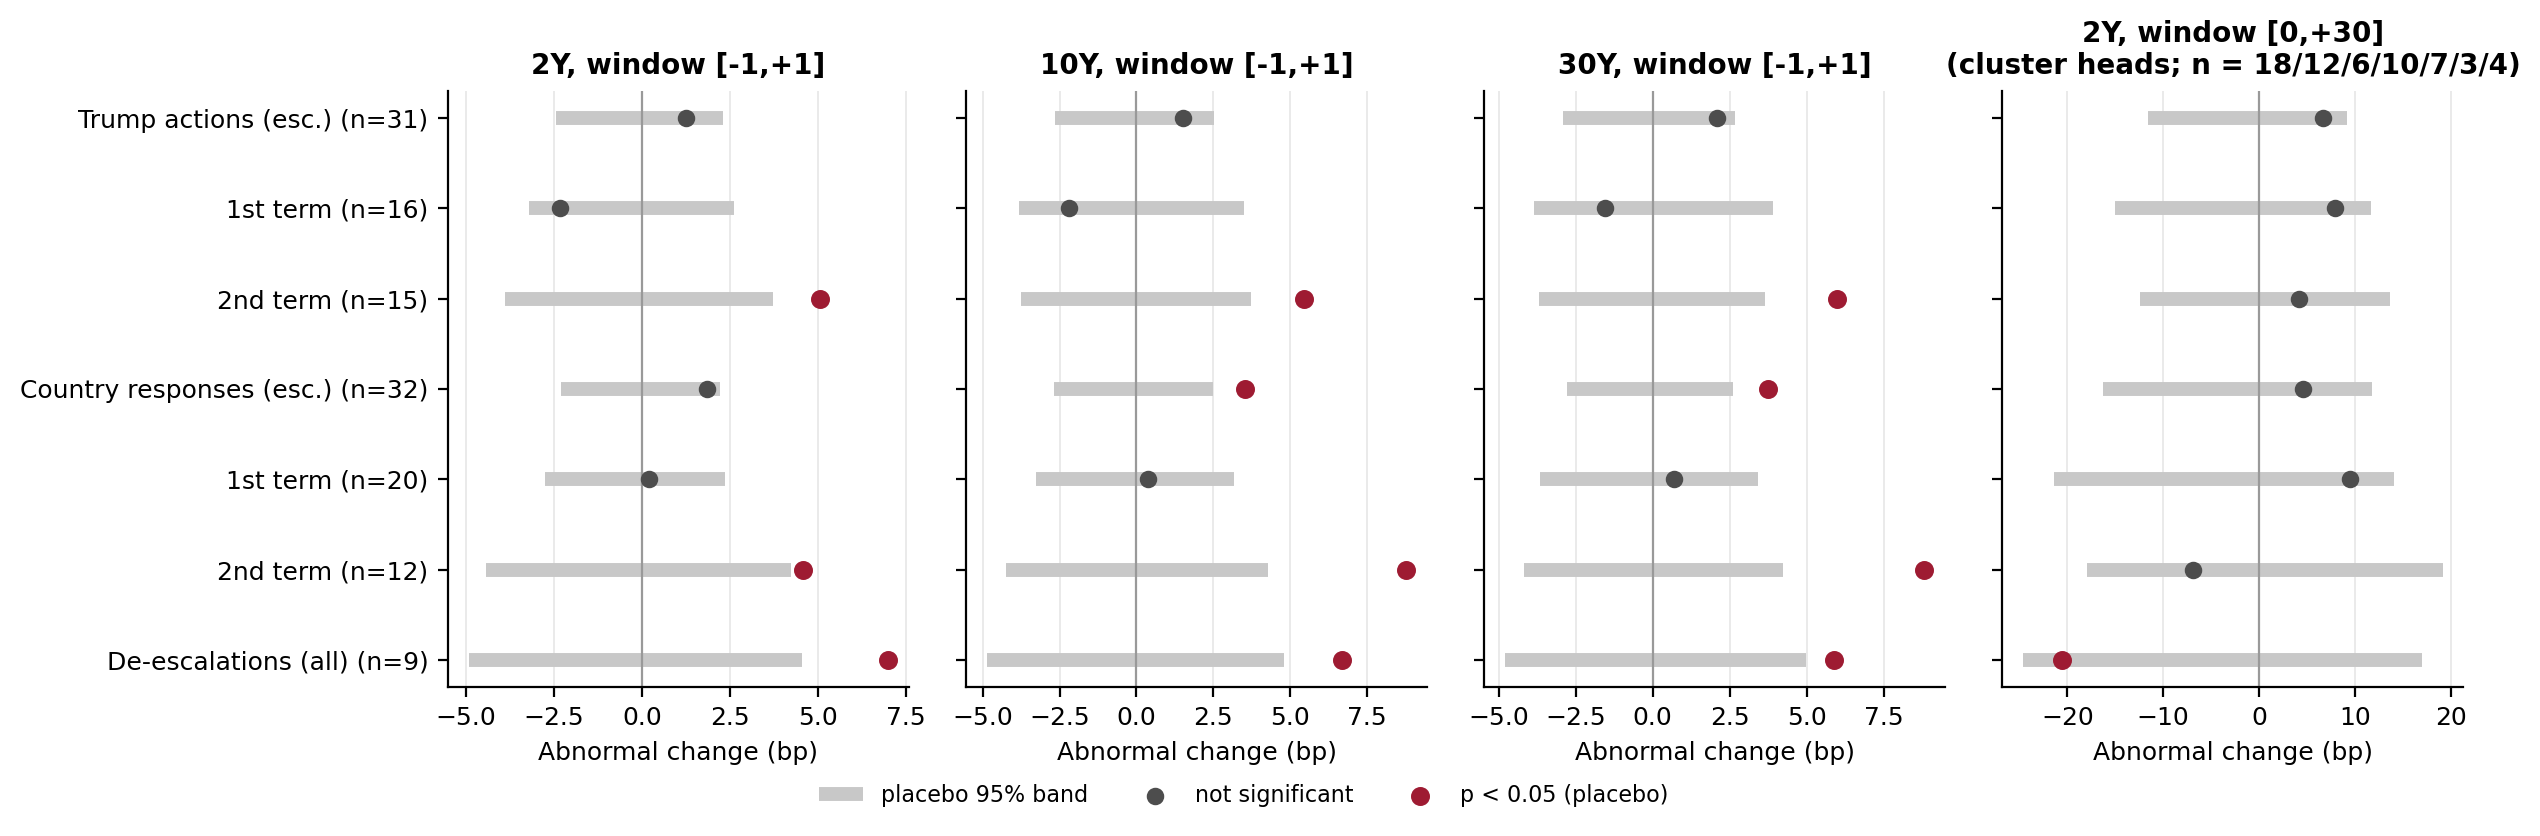
\includegraphics[width=\textwidth]{pl_q2_improved_dotplot.png}
\caption{Improved estimates (dots) against the 95\% range of the placebo
distribution (grey bars). Red dots are significant at 5\%.}
\end{figure}

\begin{table}[!htbp]
\centering
\small
\begin{tabular}{lcrrrr}
\toprule
 & & \multicolumn{2}{c}{10Y} & \multicolumn{2}{c}{30Y} \\
\cmidrule(lr){3-4}\cmidrule(lr){5-6}
2025 escalations, window $[-1,+1]$ & $n$ & bp & $p$ & bp & $p$ \\
\midrule
Trump actions, all                  & 15 & $+5.5$ & 0.005 & $+6.0$ & 0.002 \\
\quad excl.\ April 2025             & 13 & $+5.7$ & 0.006 & $+5.7$ & 0.005 \\
\quad excl.\ same-day foreign response & 12 & $+3.4$ & 0.112 & $+3.7$ & 0.072 \\
\addlinespace
Foreign responses, all              & 12 & $+8.8$ & $<0.001$ & $+8.8$ & $<0.001$ \\
\quad excl.\ April 2025             & 9  & $+6.7$ & 0.005 & $+6.7$ & 0.006 \\
\quad excl.\ same-day Trump action  & 9  & $+7.1$ & 0.004 & $+6.8$ & 0.005 \\
\bottomrule
\end{tabular}
\caption{Robustness of the 2025 announcement effect (placebo $p$-values). No
2025 escalation falls within $\pm1$ day of an FOMC decision, so that
exclusion changes nothing.}
\label{tab:rob25}
\end{table}

\begin{figure}[!htbp]
\centering
\includegraphics[width=0.95\textwidth]{pl_q2_liberation_day.png}
\caption{Daily yields around ``Liberation Day''. The announcement came after
the close on 2 April, so the reaction is on 3 April ($-20$\,bp 2Y, $-14$\,bp
10Y). From 7 to 10 April the long end sold off ($+45$\,bp on the 30Y between
the 4 and 10 April closes) while tariffs were still escalating.}
\label{fig:lib}
\end{figure}

\subsection*{(c) How the improvements change our answers to Q1}

\begin{table}[!htbp]
\centering
\footnotesize
\begin{tabular}{p{1.1cm}p{5.4cm}p{7.6cm}}
\toprule
 & Assignment design (Q1) & Improved design (Q2) \\
\midrule
Q1.1 & Abnormal declines of 10--14\,bp after Trump actions, but no
announcement effect and a raw change close to zero. &
\textbf{Confirmed: no effect when both mandates are pooled.} Trump escalations
have no significant announcement effect ($p\ge0.13$; 1 of 20 robustness
cells below 5\%). The 30-day decline disappears ($+6.6$\,bp on the 2Y, n.s.)
once each event is compared with its own rate regime. \\
\addlinespace
Q1.2 & Level down, slope up ($+4.5$\,bp): an apparent bull steepening. &
No level effect when pooled. A steepening over $[0,+5]$ ($+2.0$\,bp, $p=0.07$)
comes entirely from 2025 ($+4.6$\,bp$^{**}$), and it follows a \emph{rise} in
yields, not a front-end rally: a bear steepening. \\
\addlinespace
Q1.3 & Abnormal change near zero after responses, while raw 10Y and 30Y
yields rise by 5--7\,bp. & \textbf{Significant rise in long yields}: 10Y
$+3.5^{**}$ and 30Y $+3.7^{**}$ at the announcement, $+4.1$ to $+4.3^{**}$
over five days. The effect is entirely due to 2025 (10Y and 30Y
$+8.8^{**}$, slope $+4.2^{**}$) and survives dropping April. \\
\addlinespace
Q1.4 & 1st term: no raw reaction. 2nd term: front-end decline and
steepening. & \textbf{1st term: no effect at any horizon. 2nd term: yields
rise} by 5--6\,bp across the curve on Trump escalation days and by 9\,bp at
the long end after retaliation; the curve then steepens. The 30-day
front-end decline of 2025 is not event-specific: it is the general 2025
trend. Treasuries did not act as a safe haven. \\
\addlinespace
New & --- & \textbf{De-escalations also raise yields} ($+6$ to $+7$\,bp, with
an unchanged slope; e.g.\ $+20$\,bp on the 2Y on 9 April 2025). This is a
``risk-on'' repricing of expected Fed cuts, which pooling escalations with
de-escalations had hidden. \\
\bottomrule
\end{tabular}
\caption{Conclusions before and after the methodological improvements.}
\label{tab:before_after}
\end{table}

\textbf{Overall.} The smooth 60-day patterns of Q1 are mostly a rate-regime
effect plus clustering, not tariff news. Once these are removed, three
findings remain:
\begin{enumerate}[nosep]
\item First-term tariff news had no measurable effect on Treasury yields.
\item In 2025, escalation days, and above all foreign retaliation,
\emph{raised} yields and steepened the curve. The rise is largest at the long
end, consistent with a rising term premium (inflation, fiscal and
foreign-demand concerns) rather than a flight to safety. It is not driven by
April 2025 alone.
\item De-escalations raised yields roughly in parallel, as markets priced out
Fed cuts. The \emph{slope} separates the two channels: escalations steepen
the curve, de-escalations do not.
\end{enumerate}

\textbf{Remaining limitations.}
\begin{itemize}[nosep]
\item \textbf{Multiple testing.} Table~\ref{tab:improved} reports 84 tests,
21 of them significant at 5\%, against about 4 expected by chance. The
significant cells, however, are concentrated in the 2025 groups, whose events
fall in the same few months, so they are far from 21 independent findings.
\item \textbf{Small samples.} The second-term groups have 12--15 events in
the short windows and only 3--6 in the 30-day windows. The 30-day results,
including the $-20$\,bp for de-escalations ($n=4$), are anecdotal.
\item \textbf{Overlaps remain.} Removing same-day foreign responses weakens
the 2025 Trump effect ($p=0.07$--$0.11$), so part of it may be retaliation
news released on the same day.
\item \textbf{Daily data.} A cleaner design would use intraday Treasury
futures in 30-minute windows around each announcement, and zero-coupon rather
than par yields.
\item \textbf{Foreign curves.} With the relevant data, foreign yields could
measure the reaction in the targeted countries directly.
\end{itemize}

\end{document}
